\documentclass{elsarticle}
\biboptions{numbers,sort&compress}
\usepackage[utf8]{inputenc}
\usepackage{caption} %subfigures
\usepackage{subcaption} %subfigures
\usepackage{enumerate} % enumerados
\usepackage{listings} % listings
\usepackage{color} %colores

\definecolor{myfucsia}{rgb}{1, 0.078, 0.576}
\definecolor{mygray}{rgb}{0.941, 0.941, 0.941}
\definecolor{mypurple}{rgb}{0.109, 0.670, 0.886}
\lstset{ 
  backgroundcolor=\color{mygray},
  commentstyle=\color{myfucsia},
  keywordstyle=\color{mypurple}, 
  numberstyle=\tiny\color{myfucsia}
  stringstyle=\color{mypurple}, 
  breaklines=true,
}

\title{Simulaci\'on de estudio reol\'ogico de soluci\'on polim\'erica de carboximetil celulosa\tnoteref{t1}}
\tnotetext[t1]{Proyecto final: Simulaci\'on computacional de nanomateriales}
\author[1]{ Claudia Lizeth Hern\'andez Ram\'irez}
\ead{claudia.hernandezrmrz@uanl.edu.mx}
\date{Fall term 2021}
\address[1]{M.C. de la Ingenier\'ia con Orientaci\'on en Nanotecnolog\'ia, \\ Facultad de Ingeniería Mec\'anica y El\'ectrica, \\ Universidad Aut\'onoma de Nuevo Le\'on}
\journal{Prof.\ Schaeffer for grading}

\begin{document}

\begin{abstract}

El presente trabajo tiene como prop\'osito explicar algunas de las propiedades m\'as comunes de la \textit{Carboximetil celulosa (CMC)}; Adem\'as de simular el comportamiento de la viscosidad contra la tasa de corte de la CMC a diferentes temperaturas, adaptarlo a un modelo reol\'ogico y graficar.

Los datos obtenidos son simulados y \textit{no} deber\'an tomarse como verdaderos.
El prop\'osito de este trabajo es meramente \textit{acad\'emico}.
\end{abstract}

\begin{keyword}
reolog\'ia, tasa de corte, viscosidad, carboximetil celulosa.
\end{keyword}

\maketitle
\section{Introducci\'on}
La carboximetil celulosa (CMC) es un pol\'imero biocompatible cuyo proceso de s\'intesis consiste en modificar la macroestructura de la celulosa. La CMC es ampliamente utilizada en las industrias de alimentos y farmac\'eutica. En este trabajo se eval\'ua el comportamiento reol\'ogico de soluciones polim\'ericas de CMC, en funci\'on de la tasa de corte y de la temperatura. 

La reolog\'ia es la ciencia que estudia el flujo y la deformaci\'on de la materia. Sus aplicaciones abarcan diversas industrias, como la farmac\'eutica, del ramo alimenticio, procesamiento de pol\'imeros, pinturas, adhesivos, lubricantes, y cosm\'eticos, entre otras\cite{R1,R2,R3, R4}. Siendo la relaci\'on estructura-propiedades del material uno de los aspectos m\'as importantes para estas industrias. En este sentido, las propiedades reol\'ogicas de inter\'es son la viscosidad y la elasticidad. Sin embargo, para muchos procesos industriales relacionados con materiales polim\'ericos, las mediciones experimentales de la viscosidad, así como su control es de suma importancia, puesto que dicha propiedad es una medida relativa de todas las fuerzas que se oponen al flujo. En la industria de los pol\'imeros, una pr\'actica común es someter a dichos materiales a un proceso de flujo (deformación muy grande), lo cual se consigue llevando al pol\'imero a temperaturas superiores a su temperatura de transici\'on v\'itrea o bien mediante la utilizaci\'on de un solvente apropiado. 

Bajo este escenario, y considerando que los pol\'imeros tienen una macroestructura que se encuentra alejada del equilibrio termodin\'amico, el estudio reol\'ogico de los pol\'imeros a trav\'es de mediciones experimentales de su viscosidad es fundamental para comprender y controlar su flujo. Sin embargo, son muchos los casos, en los que un incremento de temperatura en los pol\'imeros, adem\'as de inducir un flujo, también promueven cambios irreversibles en su macroestructura (degradación t\'ermica o qu\'imica), por lo que esta alternativa debe descartarse. Por lo que disolver al pol\'imero con un solvente apropiado es una práctica recurrente\cite{R5}. En soluci\'on, las interacciones que caracterizan a la macroestructura del pol\'imero disminuyen considerablemente, favoreciéndose de esta manera el proceso de flujo, y macrosc\'opicamente el pol\'imero posee una apariencia l\'iquida. Sin embargo, su comportamiento reol\'ogico por lo general no corresponde al de un comportamiento estrictamente del tipo newtoniano. Por lo anterior, es evidente la necesidad de caracterizar las propiedades reol\'ogicas de los pol\'imeros en soluci\'on, particularmente para el caso en el que las soluciones polim\'ericas se sometan a condiciones de esfuerzos cortantes, por ejemplo, durante el bombeo y el transporte a trav\'es de tuber\'ias.\newline
En la literatura existe una variedad de trabajos\cite{R6,R7,R8,R9,R10}, en los cuales se describen los fundamentos te\'oricos requeridos para la interpretaci\'on de mediciones experimentales reol\'ogicas. A este respecto, los pol\'imeros bajo estudio que son atractivos actualmente son aquellos que son biodegradables y/o biocompatibles. Particularmente aquellos pol\'imeros que son derivados de la celulosa, el pol\'imero m\'as abundante en la naturaleza, ya que ofrecen potenciales aplicaciones en campos de la qu\'imica, la biolog\'ia y la medicina. Entre los diferentes tipos de pol\'imeros derivados de la celulosa, resalta por su capacidad hidrosoluble la carboximetil celulosa (CMC). Este pol\'imero biocompatible tiene una estructura macromolecular lineal (en forma de cadena) constituida de unidades repetitivas de glucopiranosas modificadas y unidas mediante enlaces covalentes \ref{Figura 1}. La estructura de la CMC le confiere importantes propiedades reol\'ogicas y de solubilidad en agua, que la hacen ideal para una amplia variedad de aplicaciones industriales, entre las que se encuentran como espesante, emulsificante y estabilizante. Dentro de sus aplicaciones m\'as novedosas en medicina, destaca el uso de disoluciones en forma de geles en cirug\'ias de coraz\'on, tor\'axicas y de c\'orneas\cite{R11,R12}.
\begin{figure}[htb!] % figura
    \centering
    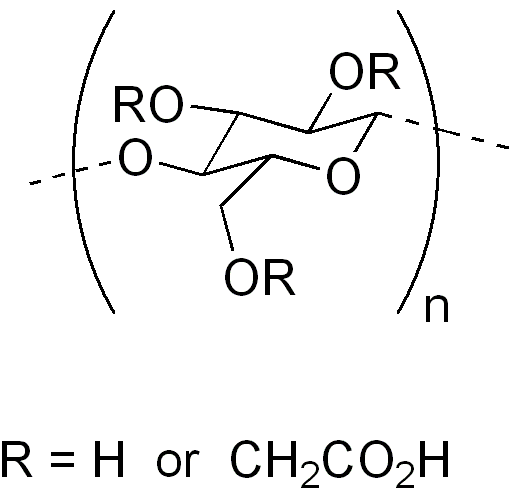
\includegraphics[width=40mm]{Carboxymethyl_cellulose.jpg} % archivo
    \caption{Estructura qu\'imica de la carboximetil celulosa.}
    \label{Figura 1}
\end{figure}

\section{Variables que modifican el valor de la viscosidad}
La viscosidad de las soluciones polim\'ericas puede afectarse significativamente por variables como la concentraci\'on de la soluci\'on, la tasa de corte o rapidez de deformaci\'on, la temperatura, la presi\'on y el tiempo\cite{R1,R5,R7}. La viscosidad tambi\'en puede ser afectada por el efecto de campos el\'ectricos o magn\'eticos, radiaci\'on UV o la humedad. El efecto de la concentraci\'on sobre la viscosidad es evidente, al aumentar la concentraci\'on de solvente la viscosidad disminuye, sin embargo, el efecto del resto de las otras variables antes mencionadas requiere de una descripci\'on con mayor detalle.\newline

\textit{El efecto de la tasa de corte}\newline
La tasa de corte es un indicador de la rapidez con que se deforma la solución polim\'erica y tiene unidades de $s^{-1}$. Actualmente en el mercado existen equipos para medir la viscosidad en rangos muy amplios de la tasa de corte ($10^4 – 10^6 s^{-1}$), seg\'un sea la aplicaci\'on. Una vez obtenidos los resultados experimentales a temperatura y presi\'on constantes del comportamiento reol\'ogico para una soluci\'on polim\'erica en particular, los cuales son la tasa de corte  ($\dot{\gamma}=\textit{d} \gamma / \textit{dt}$) y esfuerzo cortante ($\tau$), lo que prosigue es representar la informaci\'on en un gr\'afico o reograma, de manera que se pueda llevar a cabo un an\'alisis minucioso. El reograma $\tau$ vs $\dot{\gamma}$ tambi\'en conocido como curva de flujo, es el que se utiliza con mayor frecuencia y se presenta de manera esquem\'atica en la figura \ref{Figura 2}. El principal reto para el an\'alisis de estos reogramas consiste en identificar o construir la ecuaci\'on constitutiva que describa a dichos resultados experimentales\cite{R3}, ya que dicha ecuaci\'on constituye el modelo reol\'ogico (f\'isico o emp\'irico) que se debe utilizar para la interpretaci\'on de los reogramas.

\begin{figure}[h!]
\centering
\caption{Representaci\'on esquem\'atica en funci\'on de la tasa de corte.}
\begin{subfigure}[b]{0.45\linewidth}
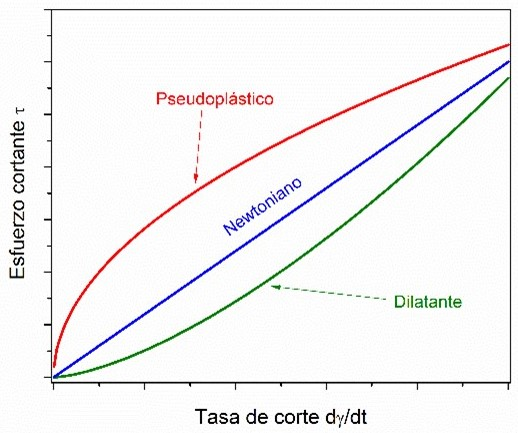
\includegraphics[width=\linewidth]{2a.jpg}
\caption{Curvas de flujo}
\label{fig:2a}
\end{subfigure}
\begin{subfigure}[b]{0.45\linewidth}
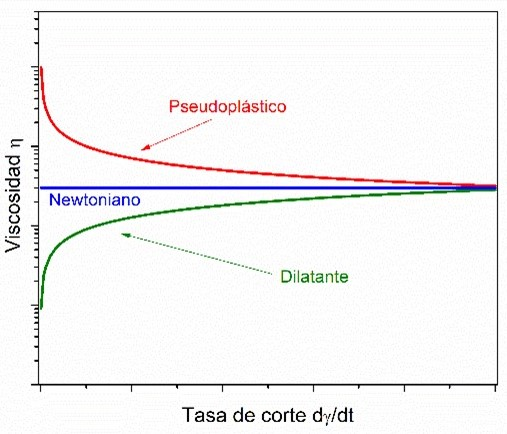
\includegraphics[width=\linewidth]{2b.jpg}
\caption{curvas de viscosidad}
\label{fig:2b}
\end{subfigure}
\label{Figura 2}
\end{figure}

Las curvas t\'ipicas de la figura \ref{fig:2a} muestran la evoluci\'on del esfuerzo cortante en funci\'on de la tasa de corte para tres comportamientos reol\'ogicos diferentes, y en la figura \ref{fig:2b} se representan las viscosidades correspondientes para estos tres casos. En estos reogramas se resumen las propiedades de flujo de la muestra bajo estudio. La interpretaci\'on de las curvas de las figuras \ref{fig:2a} y \ref{fig:2b} permite clasificar a los diferentes comportamientos reológicos previamente mencionados:
\begin{itemize}
    \item El comportamiento newtoniano corresponde a una relaci\'on lineal entre el esfuerzo cortante y la tasa de corte. Se caracteriza por presentar un valor de viscosidad (pendiente del reograma correspondiente) constante e independiente de la tasa de corte, siempre y cuando el flujo sea laminar.
    \item El comportamiento pseudopl\'astico se identifica por un reograma cuya concavidad se torna hacia abajo en la figura \ref{fig:2a}. Se caracteriza por presentar una disminuci\'on de la viscosidad a medida que aumenta la tasa de corte o rapidez de deformación, figura \ref{fig:2b}.
    \item El comportamiento dilatante se identifica por un reograma cuya concavidad se torna hacia arriba en la figura \ref{fig:2a}, lo cual se identifica en la figura \ref{fig:2b} como un incremento de la viscosidad a medida que se incrementa la tasa de corte.
\end{itemize}

\textit{El efecto de la temperatura}\newline
El efecto que tiene la temperatura sobre la viscosidad es muy significativo, pequeñas variaciones de temperatura inducen cambios importantes en la viscosidad. En la figura \ref{Figura 3} se representa de manera esquem\'atica dicho comportamiento, siempre y cuando un aumento de temperatura no produzca la creaci\'on de nuevos enlaces covalentes en la estructura del pol\'imero. La mayor\'ia de las soluciones polim\'ericas experimentan una disminuci\'on de la viscosidad a medida que se incrementa la temperatura. La relaci\'on entre la viscosidad y temperatura es compleja y se ha demostrado que, es funci\'on de la estructura, la morfolog\'ia y del tipo de interacciones f\'isicas que se desarrollen entre el solvente y el pol\'imero\cite{R13, R14}. La viscosidad de fluidos newtonianos y no-newtonianos en funci\'on de la temperatura se puede modelar de una manera muy aproximada mediante una ecuaci\'on de tipo Arrhenius:

\begin{equation}
\eta(T) = Ae^{\frac{E}{RT}}
\end{equation}

Donde \textit{T} es la temperatura absoluta, \textit{R} la constante universal de los gases (8.314 J/mol-K), \textit{E} es la energ\'ia de activaci\'on para que se d\'e el flujo y \textit{A} una constante característica de la sustancia. 

\begin{figure}[htb!] % figura
    \centering
    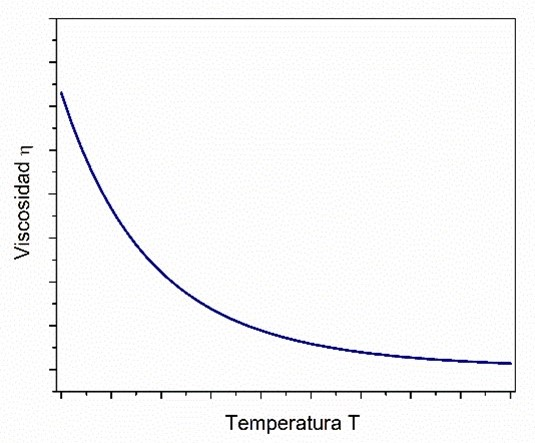
\includegraphics[width=50mm]{3.jpg} % archivo
    \caption{Representaci\'on esquem\'atica de la viscosidad en funci\'on de la temperatura para una soluci\'on polim\'erica.}
    \label{Figura 3}
\end{figure}\newpage

\section{Desarrollo}
Este proyecto fue desarrollado en \textit{RStudio} y podr\'a encontrar el c\'odigo completo en mi repositorio\cite{R15}.
Comenc\'e generando la tasa de corte que de igual forma que en la experimental,se tomaron 100 datos con un  rango de 1:1000; Se definieron los valores de \textit{A} y \textit{B} y un rango de temperaturas que son las mismas que las que se utilizaron de forma experimental con la finalidad de tener con que comparar los resultados del programa.
Se crearon dos ciclos \texttt{FOR}; uno para variar la temperatura y otro para el valor de \textit{n}.

\begin{lstlisting}[language=R, caption= Segmento de c\'odigo ciclos \texttt{FOR}.]
Tasa de corte
tasadecorte = sort(runif(100, 1, 1000))
#Datos CMC
A = 1.2606
B = -0.0211
temperatura = c(22, 30, 40, 50) #C
nqty = 1:5 #Cuantasn
aok = max(nqty) * length(temperatura)

for (temp in temperatura) {
  for (inpot in nqty) {
    n = runif(1, 0, 1) #indice de flujo n<1 =pseudoplastico n>=1 Newtoniano
    visc = ((A + (B * temp)) * tasadecorte^n-1)
    tassadecorte = c(tasadecorte)
    tazzadecorte = rep(tassadecorte, aok)
    resultado = c(temp, n, visc)
    nochidos = rbind(nochidos, resultado)
    names(nochidos) = c("Temperatura", "n", 1:100)
  }
\end{lstlisting}

Toda la informaci\'on obtenida se almacen\'o en \textit{data frames} para poder acomodar los datos de una manera apropiada.
Posteriormente se crearon dos gr\'aficas:

\begin{lstlisting}[language=R, caption= Segmento de c\'odigo boxplot.]
#BOXPLOT OK
karla$asTemperatura = as.factor(karla$asTemperatura)
ggplot(karla, aes(x = asTemperatura, y = asviscosidad,
                  fill = asTemperatura)) +
  geom_boxplot(alpha = 0.9) +
  labs(x = "Temperatura (C)", y= "Viscosidad (mPa-s)", 
       fill = "Temperatura (C)") +
  guides(fill="none")
\end{lstlisting}

\begin{lstlisting}[language=R, caption= Segmento de c\'odigo scatter plot.]
#SCATTER PLOT OK
astringente$asTemperatura = as.factor(astringente$asTemperatura)
ggplot(astringente, aes(x = asTasadecorte, y = asviscosidad, 
                        color = asTemperatura, shape = asTemperatura)) +
  geom_point(size = 3) +
  scale_color_manual(values = cols)+
  labs( x = "Tasa de corte (1/s)", y = "Viscosidad (mPa-s)",
        color = "Temperatura (C)", shape = "Temperatura (C)")
\end{lstlisting}

\begin{figure}[h!]
\centering
\caption{Reogramas de viscosidad vs tasa de corte para diferentes temperaturas.}
\begin{subfigure}[b]{0.9\linewidth}
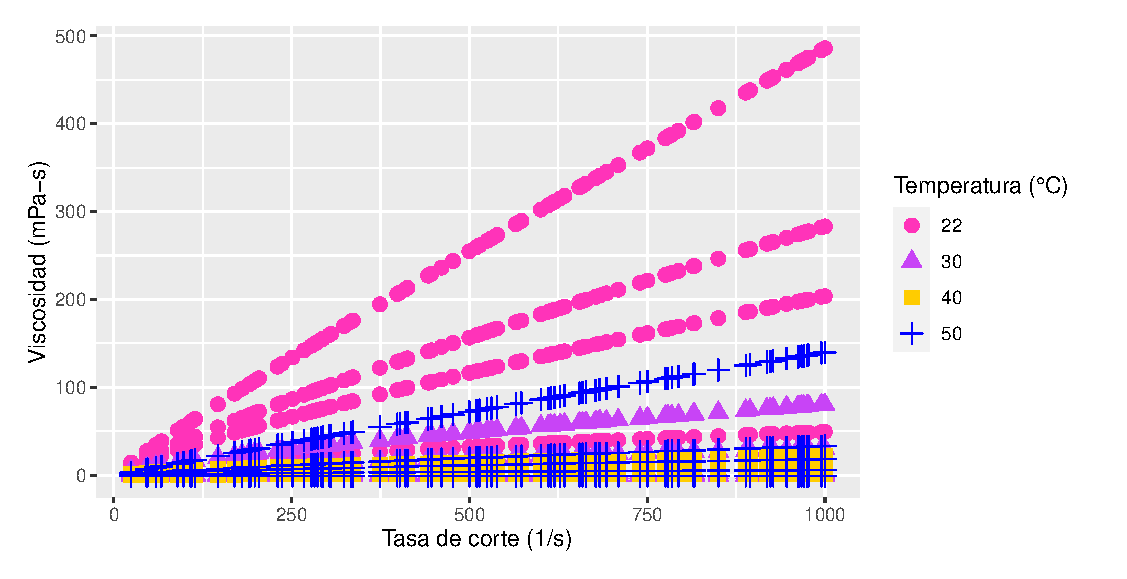
\includegraphics[width=\linewidth]{3.eps}
\caption{Prueba 1}
\label{fig:3a}
\end{subfigure}
\begin{subfigure}[b]{0.9\linewidth}
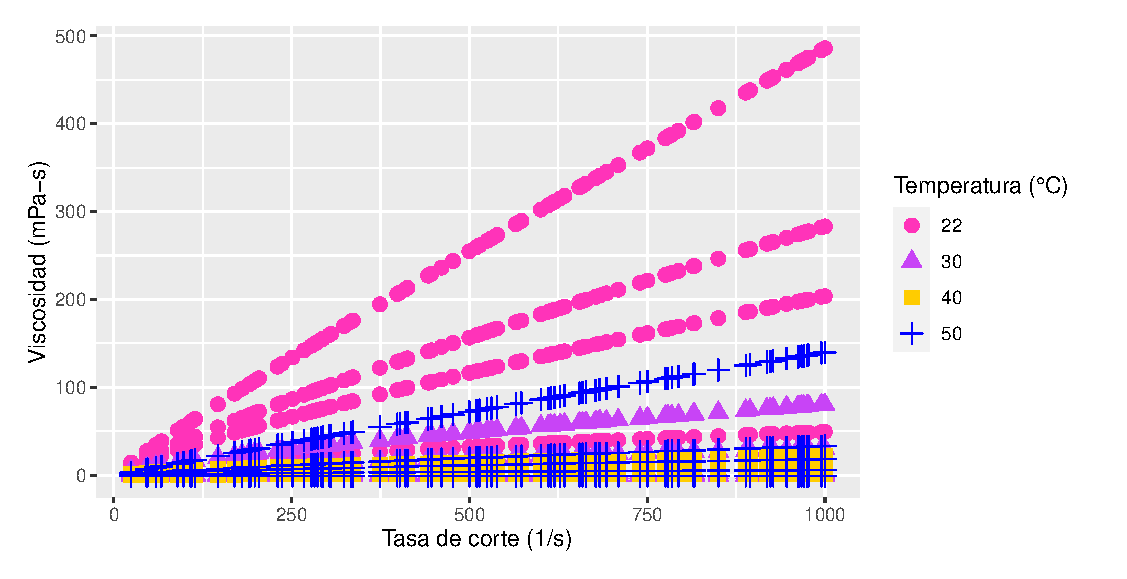
\includegraphics[width=\linewidth]{4.eps}
\caption{Prueba 2}
\label{fig:3b}
\end{subfigure}
\begin{subfigure}[b]{0.9\linewidth}
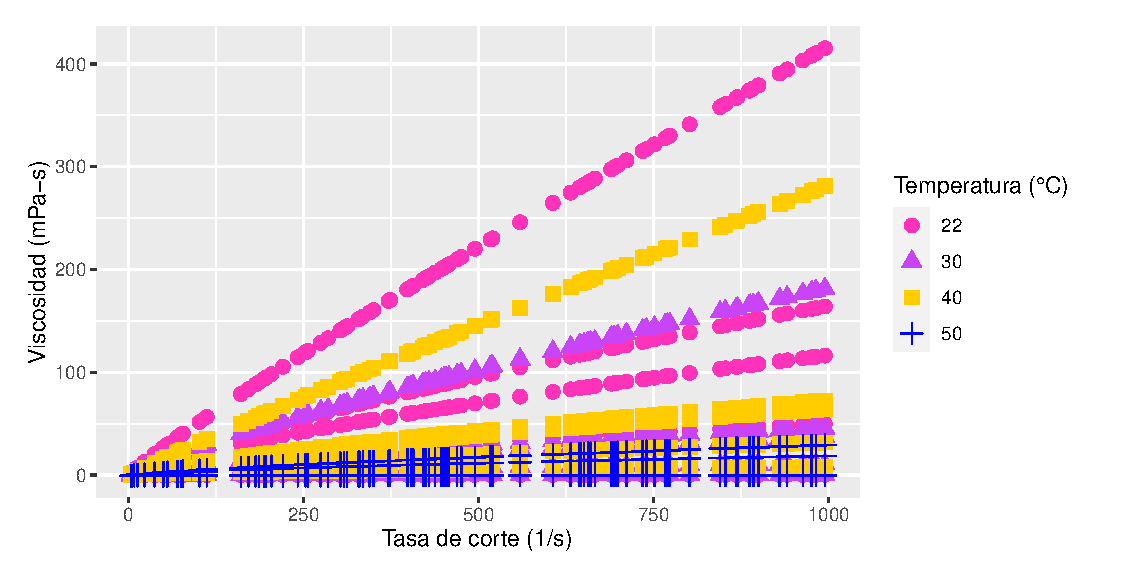
\includegraphics[width=\linewidth]{5.eps}
\caption{Prueba 3}
\label{fig:3c}
\end{subfigure}
\label{Figura 4}
\end{figure}

\begin{figure}[h!]
\centering
\caption{Boxplot de viscosidad vs tasa de corte para diferentes temperaturas.}
\begin{subfigure}[b]{0.95\linewidth}
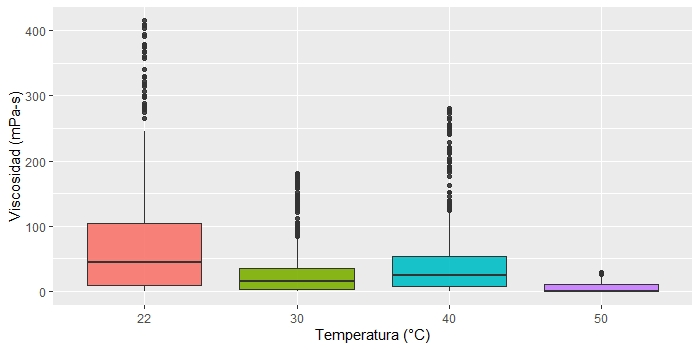
\includegraphics[width=\linewidth]{Rplot.jpeg}
\caption{Prueba 1}
\label{fig:3a}
\end{subfigure}
\begin{subfigure}[b]{0.95\linewidth}
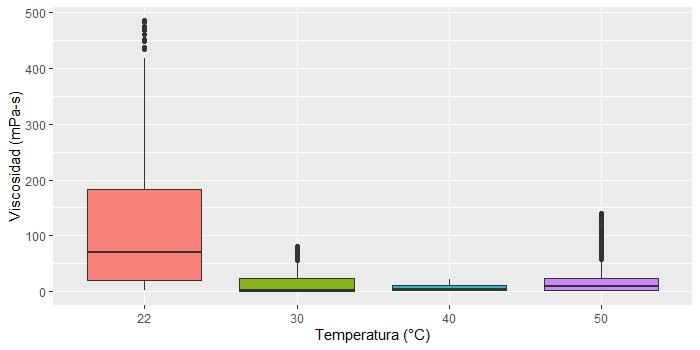
\includegraphics[width=\linewidth]{Rplot01.jpeg}
\caption{Prueba 2}
\label{fig:3b}
\end{subfigure}
\label{Figura 5}
\end{figure}
\newpage
\section{Estad\'istica}
Posteriormente apliqu\'e pruebas estad\'isticas a mis datos.
Como los resultados no fueron los esperados (lo comentar\'e en la secci\'on de conclusi\'on) agrup\'e mis datos de dos maneras; en base a la temperatura y en base al valor de \textit{n}.

\begin{lstlisting}[language=R, caption= Segmento de c\'odigo pruebas estad\'isticas agrupando por temperatura.]
#Estadistica tomando la Temperatura vs Viscosidad
tapply(astringente$asviscosidad, astringente$asTemperatura, shapiro.test)
kruskal.test(asviscosidad~asTemperatura ,astringente)
pairwise.wilcox.test(astringente$asviscosidad, astringente$asTemperatura)

astringente %>%
  group_by(asTemperatura) %>%
  summarise(
    partic = n(),
    prom = mean(asviscosidad , na.rm = TRUE),
    desv_std = sd(asviscosidad , na.rm = TRUE),
    varianza = sd(asviscosidad , na.rm = TRUE)^2,
    mediana = median(asviscosidad , na.rm = TRUE),
    ranginter =  IQR(asviscosidad , na.rm = TRUE)
  )
\end{lstlisting}

\begin{lstlisting}[language=R, caption= Segmento de c\'odigo pruebas estad\'isticas agrupando por el valor de \textit{n}.]
#Estadistica tomando la nvalue vs Viscosidad
tapply(astringente$asviscosidad, astringente$nvalue, shapiro.test)
kruskal.test(asviscosidad~nvalue ,astringente)
pairwise.wilcox.test(astringente$asviscosidad, astringente$nvalue)

astringente %>%
  group_by(nvalue) %>%
  summarise(
    partic = n(),
    prom = mean(asviscosidad , na.rm = TRUE),
    desv_std = sd(asviscosidad , na.rm = TRUE),
    varianza = sd(asviscosidad , na.rm = TRUE)^2,
    mediana = median(asviscosidad , na.rm = TRUE),
    ranginter =  IQR(asviscosidad , na.rm = TRUE)
  )
\end{lstlisting}


\section{Estad\'istica}
\begin{table}[ht]
    \centering
    \caption{Resultados obtenidos de prueba de normalidad de Shapiro, temperatura.} 
    \begin{tabular}{|r|r|r|r|}
    \hline
    K & W value & P value & ¿Se acepta H0?  \\
    \hline
    22 & 0.7766 & $2.2\times 10^{-16}$ & no \\
    \hline 
    30 & 0.7020 & $2.2\times 10^{-16}$ & no  \\
    \hline 
    40 & 0.6941 & $2.2\times 10^{-16}$ & no \\
    \hline
    50 & 0.7221 & $2.2\times 10^{-16}$ & no \\
    \hline 
\end{tabular}
    \label{cuadro 1}
\end{table}
\begin{table}[ht]
    \centering
    \caption{Resultados obtenidos de prueba de normalidad de Shapiro, \textit{n value}} 
    \begin{tabular}{|r|r|r|r|}
    \hline
    K & W value & P value & ¿Se acepta H0?  \\
    \hline
    0.0395 & 0.8338 & $3.13\times 10^{-09}$ & no \\
    \hline 
    0.0464 & 0.8368 & $4.00\times 10^{-09}$ & no  \\
    \hline 
    0.0524 & 0.8394 & $4.94\times 10^{-09}$ & no \\
    \hline
    0.2138 & 0.8974 & $1.07\times 10^{-06}$ & no \\
    \hline
    0.2169 & 0.8983 & $1.18\times 10^{-06}$ & no \\
    \hline
     0.4218 & 0.9409 & 0.0002210 & no \\
    \hline
    0.4384 & 0.9431 & 0.0003029 & no \\
    \hline
    0.5937 & 0.9568 & 0.0024160 & no \\
    \hline
    0.6016 & 0.9572 & 0.0025750 & no \\
    \hline
    0.6234 & 0.9582 & 0.0030110 & no \\
    \hline
    0.6316 & 0.9585 & 0.0031700 & no \\
    \hline
    0.6600 & 0.9594 & 0.0036730 & no \\
    \hline
    0.7220 & 0.9604 & 0.0043400 & no \\
    \hline
    0.7231 & 0.9604 & 0.0043450 & no \\
    \hline
    0.7316 & 0.9605 & 0.0043750 & no \\
    \hline
    0.7494 & 0.9605 & 0.0043890 & no \\
    \hline
    0.7727 & 0.9604 & 0.0043100 & no \\
    \hline
    0.8216 & 0.9597 & 0.0038480 & no \\
    \hline
    0.9068 & 0.9572 & 0.0025620 & no \\
    \hline
    0.9443 & 0.9556 & 0.0019970 & no \\
    \hline 
\end{tabular}
    \label{cuadro 2}
\end{table}

\begin{table}[ht]
    \centering
    \caption{Resultados obtenidos de prueba Kruskal-Wallis, temperatura.} 
    \begin{tabular}{|r|r|r|}
    \hline
    Chi cuadrada & DF & P  \\
    \hline
    649.72 & 3 & $2.2\times 10^{-16}$ \\
    \hline
\end{tabular}
    \label{cuadro 3}
\end{table}
\begin{table}[ht]
    \centering
    \caption{Resultados obtenidos de prueba Kruskal-Wallis, \textit{n value}.} 
    \begin{tabular}{|r|r|r|}
    \hline
    Chi cuadrada & DF & P  \\
    \hline
    1659.30 & 19 & $2.2\times 10^{-16}$ \\
    \hline
\end{tabular}
    \label{cuadro 4}
\end{table}

\begin{table}[htb]
    \centering
    \caption{Diferencias entre grupos. Pairwise Wilcox, temperatura} 
    \begin{tabular}{|r|r|r|r|r|}
    \hline
    "" & 22 & 3 & 4 \\
    \hline
    30 & $2.2\times 10^{-16}$ & "" & "" \\
    \hline
    40 & $2.7\times 10^{-5}$ & $3.5\times 10^{-10}$  & "" \\
    \hline
    50 & $2.2\times 10^{-16}$ & $2.2\times 10^{-16}$ & $2.2\times 10^{-16}$ \\
    \hline
    \end{tabular}
    \label{cuadro 5}
\end{table}

\begin{table}[htb]
    \centering
    \caption{Informaci\'on individual de los datos, temperatura.} 
    \begin{tabular}{|r|r|r|r|r|r|r|}
    \hline
    Carga & Participantes & Promedio & Desv. Std. & Varianza & Mediana & R. Intercuartil  \\
    \hline
    22 & 500 & 75.80 & 91.30 & 8339.00 & 44.60 & 95.70 \\
    \hline
    30 & 500 & 29.20 & 40.80 & 1666.00 & 14.50 & 31.50 \\
    \hline
    40 & 500 & 45.70 & 59.70 & 3563.00 & 25.10 & 46.10 \\
    \hline
    50 & 500 & 04.82 & 07.97 & 0063.50 & -0.16 & 10.40 \\
    \hline
\end{tabular}
    \label{cuadro 6}
\end{table}

\begin{table}[htb]
    \centering
    \caption{Informaci\'on individual de los datos, \textit{n value}.} 
    \begin{tabular}{|r|r|r|r|r|r|r|}
    \hline
    \textit{n value} & Participantes & Promedio & Desv. Std. & Varianza & Mediana & R. Intercuartil  \\
    \hline
    0.0395 & 100 & -0.74 & 0.011 & 0.000128 & -0.73 & 0.012 \\
    \hline
    0.0465 & 100 & -0.17 & 0.042 & 0.001760 & -0.16 & 0.044 \\
    \hline
    0.0525 & 100 & 00.07 & 0.061 & 0.003830 & 0.090 & 0.066 \\
    \hline
    0.2140 & 100 & -0.27 & 0.147 & 0.021600 & -0.24 & 0.183 \\
    \hline
    0.2170 & 100 & -0.26 & 0.151 & 0.022900 & -0.23 & 0.190 \\
    \hline
    0.4220 & 100 & 06.75 & 2.690 & 7.260000 & 07.08 & 3.840 \\
    \hline
    0.4038 & 100 & 04.70 & 2.040 & 4.150000 & 04.93 & 2.930 \\
    \hline
    0.5940 & 100 & 21.40 & 9.950 & 99.00000 & 21.90 & 15.20 \\
    \hline
    0.6020 & 100 & 28.80 & 13.40 & 179.0000 & 29.40 & 20.50 \\
    \hline
    0.6230 & 100 & 25.90 & 12.40 & 153.0000 & 26.40 & 19.10 \\
    \hline
    0.6320 & 100 & 17.80 & 08.73 & 76.20000 & 18.10 & 13.50 \\
    \hline
    0.6600 & 100 & 10.10 & 05.30 & 28.10000 & 10.20 & 08.26 \\
    \hline
    0.7220 & 100 & 15.30 & 08.30 & 68.90000 & 15.30 & 13.10 \\
    \hline
    0.7230 & 100 & 62.70 & 32.40 & 1051.000 & 62.60 & 51.30 \\
    \hline
    0.7320 & 100 & 34.20 & 18.00 & 325.0000 & 34.00 & 28.60 \\
    \hline
    0.7490 & 100 & 38.30 & 20.50 & 420.0000 & 38.00 & 32.60 \\
    \hline
    0.7730 & 100 & 86.00 & 46.30 & 2143.000 & 84.80 & 74.00 \\
    \hline
    0.8220 & 100 & 92.20 & 51.70 & 2673.000 & 90.00 & 83.30 \\
    \hline
    0.9070 & 100 & 202.0 & 120.0 & 14381.00 & 192.0 & 195.0 \\
    \hline
    0.9440 & 100 & 133.0 & 81.70 & 6683.000 & 126.0 & 134.0 \\
    \hline
\end{tabular}
    \label{cuadro 7}
\end{table}

\clearpage
\section{Resultados}
Es evidente que a temperaturas menores la viscosidad toma un valor mayor y por el contrario, entre mayor sea la temperatura, la viscosidad tendr\'a un menor valor; Esto puede observarse en la figura \ref{cuadro 4}; los puntos rosas que son a \textit{22°C} tienen una relacion lineal positiva.
En la figura \ref{Figura 5} podemos notar que los valores de viscosidad que se logran a altas temperaturas son notablemente menores.
Y con las pruebas estad\'isticas podemos concluir que ni la temperatura ni el valor de \textit{n} tienen un efecto significativo en la viscosidad.

\section{Conclusi\'on}
Los resultados no fueron los esperados; a menores temperaturas la viscosidad deber\'ia ser menor (como est\'a comprobado experimentalmente)\cite{R16}.
Esta discrepancia la puedo atribuir a que los valores de \textit{n} no estan correctamente calculados, solo est\'an generados con \textit{runif} cuando deber\'ian estar calculados con una f\'ormula, en la pr\'actica \textit{n} deber\'ia tener valores menores a menor temperatura.
Por otro lado, el calculo de la viscosidad requiere de mas f\'ormulas, sin embargo no fueron incluidas por fines de practicidad.

\section{Comentarios personales}
El desarrollo de este proyecto fue muy desafiante, ya que puse a prueba lo aprendido durante 6 meses de practicas semanales. Aunque estoy contenta con lo logrado, me gustar\'ia seguir trabajando con este c\'odigo con el fin de hacer un simulador que pueda servir y utilizarse en clases de licenciatura, lo tomar\'e como un proyecto secundario a mi tesis, asesor\'andome con expertos en temas de reolog\'ia, pol\'imeros y por supuesto programadores m\'as experimentados.

\bibliography{mybibfile}
\bibliographystyle{elsarticle-num-names}
\end{document}